\documentclass[a4paper,12pt]{article}

\usepackage[utf8]{inputenc}
\usepackage[T1]{fontenc}
\usepackage{amsmath}
\usepackage{verbatim}
\usepackage{array}
\usepackage{hyperref}
%\hypersetup{
%    colorlinks,
%    citecolor=black,
%    filecolor=black,
%    linkcolor=black,
%    urlcolor=black
%}
\usepackage{amssymb}
\usepackage{sectsty}
\usepackage{graphicx}
\usepackage{listings}

\sectionfont{\fontsize{26}{26}\selectfont}
\subsectionfont{\fontsize{19}{19}\selectfont}

\newtheorem{thm}{Teorem}[subsection]
\newtheorem{lem}[thm]{Lema}
\newtheorem{cor}[thm]{Korolar}
\newtheorem{defn}[thm]{Definicija}
\newtheorem{rem}[thm]{Napomena}
\newtheorem{prop}[thm]{Propozicija}
\newtheorem{exa}[thm]{Primjer}
\newtheorem{conj}[thm]{Slutnja}
\newenvironment{proof}{\textit{Dokaz.}}{\hfill}

\renewcommand{\contentsname}{Sadržaj}

\setcounter{section}{-1}


\begin{document}

\begin{titlepage}
    \centering
    \vspace*{\fill}
    %\vspace*{0.5cm}
    \huge\bfseries
    Izračunljivost u $\lambda$-računu \\ \small(seminar)
    \vspace*{0.5cm}

    \small Sandro Lovnički
    \vspace*{\fill}
\end{titlepage}

\tableofcontents % show correctly after 2nd build
\newpage

\section{Uvod}

\qquad Cilj ovog rada je pokazati kako je $\lambda$-račun jedan od mogućih modela za opisivanje izračunljivosti. To ćemo učiniti eksplitinim definiranjem inicijalnih funkcija unutar $\lambda$-računa te provođenjem dokaza zatvorenosti $\lambda$-definabilnih funkcija na kompoziciju, primitivnu rekurziju i minimizaciju. Kao glavni rezultat toga, slijedit će Kleenejev teorem o ekvivalenciji parcijalno rekurzivnih funkcija te $\lambda$-definabilnih funkcija.\\
Nadalje, u konkretnoj implementaciji interpretera za $\lambda$-račun, pokazat ćemo i kako zaista djeluju apstraktni $\lambda$-izrazi koji stvaraju primitivne rekurzije i minimizacije. Kao primjere programskih kodova dat ćemo izgradnje nekih klasičnih primjera rekurzivnih funkcija.

\subsection{Osnovne definicije $\lambda$-računa}

U ovom uvodnom potpoglavlju, dat ćemo kratak podsjetnik na osnovne definicije $\lambda$-računa, ali rad podrazumijeva da je čitatelj upoznat s $\lambda$-računom te će većina stvari biti korištena u skladu s tim. Često će u dokazima biti korišteni $\lambda$-izrazi koji možda nisu prije toga eksplicitno definirani, ali čija uloga je jasna.

\begin{defn} Lambda izrazi su riječi nad abecedom koju čine:
\begin{itemize}
	\item varijable: $v_0$,$v_1$,$...$
	\item apstraktor: $\lambda$
	\item zagrade i točka: $($,$)$,$.$
\end{itemize}
\end{defn}

\begin{defn} Skup $\lambda$-izraza $\Lambda$ definiramo induktivno:
\begin{itemize}
	\item $x \in \Lambda$, gdje je $x$ varijabla
	\item $M \in \Lambda \Rightarrow \lambda x.M \in \Lambda$
	\item $M,N \in \Lambda \Rightarrow (MN) \in \Lambda$
\end{itemize}
\end{defn}

\begin{rem} Navedimo ovdje i neke notacijske napomene koje će nam olakšati pisanje i razumijevanje:
\begin{enumerate}
	\item varijable ćemo označavati malim slovima (x,y,z,...), a $\lambda$-izraze velikim (M,N,...)
	\item vanjske zagrade nećemo pisati
	\item $\overrightarrow{x} \equiv x_1, ..., x_n$, $\overrightarrow{N} \equiv N_1, ..., N_n$
	\item $\lambda \overrightarrow{x}.M \equiv \lambda x_1. \lambda x_2. ... \lambda x_n. M$
	\item M$\overrightarrow{N}$ $\equiv$ $(... ((MN_1) N_2) ...N_n)$ (asocijativnost ulijevo)
\end{enumerate}
\end{rem}

\begin{defn} (Supstitucija) Kažemo da je $N$ supstituiran za $x$ u $M$ i pišemo $M[x:=N]$ ako smo sve odgovarajuće pojave varijable $x$ u izrazu $M$ zamijenili izrazom $N$.
\end{defn}

\begin{defn} Teorija $\lambda$ ima formule oblika M = N (M,N $\in$ $\Lambda$) generirane sljedećim aksiomima i pravilima:
\begin{enumerate}
	\item $(\lambda x.M)N = M[x:=N]$ ($\beta$-konverzija)
	\item $M = M$
	\item $M = N \Rightarrow N = M$
	\item $M = N, N = L \Rightarrow M = L$
	\item $M = N \Rightarrow MZ = NZ$
	\item $M = N \Rightarrow ZM = ZN$
	\item $M = N \Rightarrow \lambda x.M = \lambda x.N$
	\item $\lambda x. M x = M$ ($\eta$-konverzija)
\end{enumerate}
\end{defn}

\newpage
%%%%%%%%%%%%%%%%%%%%%%%%%%%%%%%%%%%%%%%%%%%%%%%%%%%%%%%%%%%%%%%%%%%%%%%%%%%%%%%%%%%%%%%%%%%%%%%%%%%%%%
%
%		SECTION 1
%
%%%%%%%%%%%%%%%%%%%%%%%%%%%%%%%%%%%%%%%%%%%%%%%%%%%%%%%%%%%%%%%%%%%%%%%%%%%%%%%%%%%%%%%%%%%%%%%%%%%%%%

\section{Rekurzivnost i $\lambda$-definabilnost}

Bez obzira koji model izračunavanja koristimo (RAM-programe, Turingov stroj, $\lambda$-račun, Postove strojeve, ...), definabilnost se bavi definiranjem funkcija unutar danog modela što za cilj ima pokazati koliko je taj model robustan.
\\\\
Glavna točka ovog poglavlja je pokazati ekvivalenciju skupa funkcija koje je moguće definirati unutar $\lambda$-računa i skupa parcijalno rekurzivnih funkcija. Sjetimo se, skup parcijalno rekurzivnih funkcija sastoji se od svih inicijalnih funkcija te je zatvoren na kompoziciju, primitivnu rekurziju i minimizaciju.

\subsection{Churchovi numerali}

Kako skup $\Lambda$ eksplicitno ne sadrži nikakve numerale (reprezentacije apstraknog pojma broja), htjeli bismo odabrati $\lambda$-izraze koji će ih reprezentirati. Nadalje, želimo definirati i brojevne funkcije nad takvim numeralima. Koristiti ćemo najpoznatiju verziju numerala unutar $\lambda$-računa - Churchove numerale.

\begin{defn} Definiramo $c_n = c_0,c_1,...$, gdje je
	\[ c_n = \lambda f x. f^n x  = \lambda f x. f (f ... (f x) ...) \]
\end{defn}
%
Dakle, broj $n$ reprezentiramo numeralom $c_n$ koji prima $f$ i $x$ te vraća vrijednost izraza dobivenog $n$ puta primjenom $f$ na $x$.
\\\\
Jasno, nisu sve numeričke funkcije definirane na cijeloj svojoj domeni te izračunavanje takvih nikad ne stane. Kako bismo i tu opciju imali pokrivenu $\lambda$-izrazima, uvedimo sljedeću definiciju.

\begin{defn} Kažemo da je $M \in \Lambda$ rješiv ako $\exists \overrightarrow{N}$ takvi da je $M \overrightarrow{N} = I$. Ako $M$ nije rješiv, kažemo da je nerješiv.
\end{defn}

\begin{lem} Svi Churchovi numerali su rješivi $\lambda$-izrazi i to za $\overrightarrow{N}$ (iz definicije) $= I I$.
\end{lem}
\begin{proof} Indukcijom.
\begin{itemize}
	\item $c_0 I I = (\lambda f x. x) I I = (\lambda x. x) I = I$
	\item $c_{n+1} I I = (S c_n) I I = ((\lambda n f x. f (n f x)) c_n) I I = (\lambda f x. f (c_n f x)) I I =\\= (\lambda x. I (c_n I x)) I = I (c_n I I) = (pretp.) = I I = I$
\end{itemize}
\end{proof}

\subsection{Y kombinator}

Implementacija rekurzije (koja će nam trebati u sljedećem potpoglavlju) samopozivanjem nije dopuštenja u $\lambda$-računu stoga moramo posegnuti za najznačajnijom idejom u teoriji programskih jezika. Konstruirat ćemo $\lambda$-izraz $Y$ koji će, primijenjen na nerekurzivnu funkciju $f$, kreirati njenu "rekurzivnu verziju" tražeći joj fiksnu točku. $Y$ kombinator zovemo i kobinator fiksne točke.

\begin{defn} $Y := \lambda f.(\lambda x.f(x x))(\lambda x.f(x x))$.
\end{defn}

\begin{prop} $Y$ kombinator je kombinator fiksne točke, tj. 
	\[ YF = F(YF),\ \forall F \in \Lambda \]
\end{prop}
\begin{proof} Neka je $W := \lambda x. F (x x)$. Tada je
	\[ YF = WW = (\lambda x. F (x x)) W = F(WW) = F(YF) \]
\end{proof}
\begin{rem} Kombinatora fiksne točke ima prebrojivo mnogo. 
\end{rem}
~\\
Uzmimo za primjer funkciju $fakt$ za koju želimo da prima numeral $c_n$ i rekurzivno računa te vraća $c_{n!}$. Intuitivna definicija funkcija faktorijela dana je s
	\[ fakt := \lambda n.\ if\ (eq\ n\ c_0)\ c_1\ (mul\ n\ (fakt\ (pred\ n))) \]
Kao što smo rekli, samopozivanje nije dopuštano pa apstrahirajmo $fakt$ u tijelu funkcije.
	\[ fakt' := \lambda f n.\ if\ (eq\ n\ c_0)\ c_1\ (mul\ n\ (f\ (pred\ n))) \]
Ovakva definicija sad je dopustima u $\lambda$-računu, ali izgubili smo svojstvo rekurzivnosti.

\begin{lem} Funkcija $faktorijel := Y\ fakt'$ rekurzivno računa faktorijel, tj. $faktorijel\ c_n = c_{n!}$
\end{lem}
\begin{proof} Primijetimo da je definicija dopustiva u $\lambda$-računu jer ne sadrži eksplicitno samopozivanje.\\
Dokaz provodimo indukcijom. Za lakše čitanje dokaza, označimo $yf := \lambda x. fakt' (x x)$. Primijetimo da je tada $Y\ fakt' = yf\ yf = fakt'\ (yf\ yf)$.
\begin{itemize}
	\item $c_0$.
		\[ faktorijel\ c_0 = (Y\ fakt')\ c_0 = fakt'\ (yf\ yf)\ c_0 = \] 
		\[ = if\ (eq\ c_0\ c_0)\ c_1\ (mul\ c_0\ ((yf\ yf)\ (pred\ c_0))) = c_1 \]
	\item Neka tvrdnja vrijedi za neki $c_n$, tj. $faktorijel\ c_n = c_{n+1}$. Tada imamo (uz početak sličan kao gore)
		\[ faktorijel\ c_{n+1}\ = ... = \]
		\[ = if\ (eq\ c_{n+1}\ c_0)\ c_1\ (mul\ c_{n+1}\ ((yf\ yf)\ (pred\ c_{n+1}))) = \]
		\[ = mul\ c_{n+1}\ (fakt'\ (yf\ yf)\ (pred\ c_{n+1})) = \] 
		\[ = mul\ c_{n+1}\ (faktorijel\ c_n) = (pretp.) =  mul\ c_{n+1}\ c_{n!} = c_{(n+1)!} \] 
\end{itemize}
Iz dokaza koraka indukcije vidimo da $faktorijel$ zaista računa na rekurzivan način.
\end{proof}

\subsection{$\lambda$-definabilnost}

$\lambda$-račun predstavlja određenu klasu funkcija nad prirodnim brojevima. Pokazat će se, po rezultatu Kleeneja, da su to upravo parcijalno rekurzivne funkcije. Krenimo sad s dokazima koji će voditi tom rezultatu.

\begin{defn}
Neka je $\varphi$ parcijalna numerička funkcija s $p$ argumenata. Kažemo da je $\varphi$ $\lambda$-definabilna ako postoji $F \in \Lambda$ takav da $\forall \overrightarrow{n} \in \mathbb{N}$
\begin{center}
$\begin{cases}
F \overrightarrow{c_n} = c_{\varphi (\overrightarrow{n})},& \varphi (\overrightarrow{n}) \mbox{ je definirana u } \overrightarrow{n}\\
F \overrightarrow{c_n} \mbox{ je nerješiv},& \mbox{inače}
\end{cases}$
\end{center}
Eksplicitno kažemo i da je $\varphi$ $\lambda$-definirana s $F$.
\end{defn}

\begin{lem}
Incijalne funkcije su $\lambda$-definabilne.
\end{lem}
\begin{proof} Definirajmo odgovarajuće $\lambda$-izraze za nul-funkciju, projekciju i sljedbenika.
\begin{itemize}
	\item $Z := \lambda x. c_0 $\\
		Trivijalno.
	\item $I^k_n := \lambda x_1, ..., x_k . x_n$\\
		Trivijalno.
	\item Neka je $f$ $\lambda$-izraz koji predstavlja funkciju sljedbenika i neka $x$ predstavlja nulu. Tada bi, po definiciji Churchovih numerala, $c_n f x$ bio broj $n$, a njegov sljedbenik $n+1$ bi tada bio $f(c_n f x)$. Dakle, $c_{n+1} f x = f (c_n f x)$. Ako sad apstrahiramo $f$ i $x$ na obje strane, imamo $\lambda f x. c_{n+1} f x = \lambda f x. f (c_n f x)$. Na lijevoj strani iskoristimo aksiom $\eta$-konverzije da bismo dobili $c_{n+1} = \lambda f x. f (c_n f x)$ te sad apstrahiramo $c_n$ da bismo dobili funkciju sljedbenika:
	\[ S := \lambda n f x . f (n f x) \]
		Zaista, $S c_n = (\lambda n f x . f (n f x)) c_n = \lambda f x. f (c_n f x) =\\= \lambda f x. f (\lambda f x. f (f ... (f x) ...)) f x) = \lambda f x. f (f (f ... (f x) ...))) = c_{n+1}$.
\end{itemize}
\end{proof}
\\
Kad govorimo o $\lambda$-definabilnosti kompozicije parcijalnih funkcija, valja biti oprezan. Naime, reprezentacija kompozicije nije uvijek jednaka kompoziciji reprezentacija funkcija članica što možemo vidjeti kroz sljedeći primjer.

\begin{exa} Neka je $\forall n$ $f(n)=0$ i $g(n)$ nedefinirana. Tada je njihova kopozicija $f \circ g$ nedefinirana za svaki $n$. Ove funkcije možemo definirati $\lambda$-izrazima $F = \lambda x. c_0$ i $G = \lambda x. \Omega$, ali tada imamo
	\[ F G = (\lambda x. c_0) G = c_0 \]
što svakako nije nerješiv izraz.
\end{exa}

\begin{lem} $\lambda$-definabilne parcijalne funkcije zatvorene su na kompoziciju.
\end{lem}
\begin{proof} Neka su $\chi, \psi_1 ,..., \psi_m$ $\lambda$-definirane s $G, H_1 ,..., H_m$, respektivno.\\ Tada je
    \[ \varphi (\overrightarrow{n}) \simeq \chi (\psi_1 (\overrightarrow{n}), ..., \psi_m (\overrightarrow{n})) \]
$\lambda$-definirana s
    \[ F \equiv \lambda \overrightarrow{x}.(H_1 \overrightarrow{x}II)  ... (H_m \overrightarrow{x}II) (G(H_1 \overrightarrow{x}) ... (H_m \overrightarrow{x})) \]
Lako je za vidjeti da takav $F$ zaista zadovoljava definiciju.
\end{proof}
\\
\begin{lem} $\lambda$-definabilne funkcije zatvorene su na primitivnu rekurziju.
\end{lem}
\begin{proof} Neka su $\chi$ i $\psi$ $\lambda$-definirane s G i H, respektivno.\\
Tada je $\varphi$ definirana s
    \[ \varphi (\overrightarrow{n}, 0) = \chi ( \overrightarrow{n}) \]
	\[ \varphi (\overrightarrow{n}, k+1) = \psi (\overrightarrow{n},k,\varphi (\overrightarrow{n},k)) \]
$\lambda$-definirana s
	\[ F \equiv \lambda \overrightarrow{x}.\ Y\ (\lambda f \overrightarrow{x} k.\ (isZ\ k)\ (G \overrightarrow{x})\ (H\ \overrightarrow{x}\ (pred\ k)\ (f\ \overrightarrow{x}\ (pred\ k)))) \]
Indukcijom po $k$, vidi se da je $F \overrightarrow{c_n} k = c_{\varphi (\overrightarrow{n},k)}$.
\end{proof}
\\
\begin{lem} $\lambda$-definabilne funkcije zatvorene su na minimizaciju.
\end{lem}
\begin{proof} Neka je je $\chi$ totalna funkcija $\lambda$-definirana s $G$ i 
	\[ \varphi(\overrightarrow{n}) \simeq \mu m [\chi(\overrightarrow{n},m) = 0] \]
Kao pomoćnu funkciju, za neki $P \in \Lambda$ za koji vrijedi ili $P c_n = T$ ili $P c_n = F$ za sve $n$, definirajmo $H_p = Y (\lambda h z.\ Pz\ z\ (h\ (S\ z)))$. Sad minimizaciju izraza $P$ možemo zapisati kao slanje početne vrijednosti $z=0$ rekurzivnom evaluatoru $H_p$, tj. $\mu P = H_p c_0$.\\
Analogno, (za $P = \lambda y.\ isZ\ (G \overrightarrow{x} y)$) izraz definiran s
	\[ F \equiv \lambda \overrightarrow{x}.\ \mu[\lambda y.\ isZ\ (G \overrightarrow{x} y)] \]
$\lambda$-definira $\varphi$.
\end{proof}
\\
\begin{prop} Parcijalno rekurzivne funkcije su $\lambda$-definabilne.
\end{prop}
\begin{proof}
Slijedi iz dokaza prethodnih lema.
\end{proof}
\\
\begin{thm} (Kleene) Parcijalna funkcija je parcijalno rekurzivna ako i samo ako je $\lambda$-definabilna.
\end{thm}

 

\newpage
%%%%%%%%%%%%%%%%%%%%%%%%%%%%%%%%%%%%%%%%%%%%%%%%%%%%%%%%%%%%%%%%%%%%%%%%%%%%%%%%%%%%%%%%%%%%%%%%%%%%%%
%
%		SECTION 2
%
%%%%%%%%%%%%%%%%%%%%%%%%%%%%%%%%%%%%%%%%%%%%%%%%%%%%%%%%%%%%%%%%%%%%%%%%%%%%%%%%%%%%%%%%%%%%%%%%%%%%%%

\section{pLam}
Kako bismo konstruirane ideje iz prethodnih poglavlja testirali, poslužit ćemo se interpreterom za $\lambda$-račun napisanom u Haskellu. Izračunavanje rekurzivnih funkcija vidjet ćemo na primjerima programa napisanih u jeziku čistog $\lambda$-računa, koji intepreter pLam prepoznaje. \\
\\
Kompletan izvorni kod ovog interpretera, kao i upute za njegovo korištenje, mogu se naći na adresi \href{https://github.com/sandrolovnicki/lambda-calculus-interpreter}{https://github.com/sandrolovnicki/lambda-calculus-interpreter}. 

%=================================================================================================================

\subsection{Biblioteka $comp$}
Jasno je da konstrukcija iole kompliciranijih izračunavanja zahtijeva postojanje predefiniranih bazičnih i raznih pomoćnih funkcija kako ne bismo svaki puta morali pisati mnogo redaka $\lambda$-izraza, već samo nekoliko ključnih. To će nam biti omogućeno naredbom $:import\ libname$, gdje su u $import/libname.plam$ definirani željeni $lambda$-izrazi.\\

\begin{figure}[h]
\centering
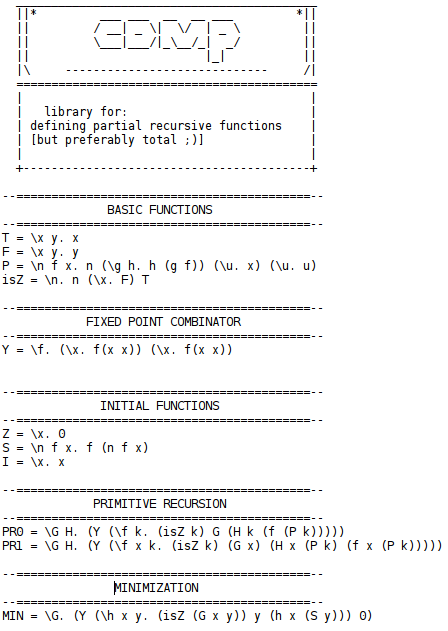
\includegraphics[width=0.5\textwidth]{comp}
\caption{Slika biblioteke $comp$}
\end{figure}


\subsection{Primjeri}

\begin{lstlisting}
         _
        | |
    ____| |   ___  __  __
    | _ \ |__| _ \|  \/  |
    |  _/____|____\_\__/_| v0.1.0
    |_| pure lambda-calculus interpreter
   =================================

pLam> -- defining factorial as primitive recursion of 1 and mul
pLam>
pLam> :import std
pLam> :import comp
pLam> 
pLam> factorial = PR0 1 mul
pLam> 
pLam> factorial 3
----- result: 6
pLam> 

\end{lstlisting}

\begin{lstlisting}
         _
        | |
    ____| |   ___  __  __
    | _ \ |__| _ \|  \/  |
    |  _/____|____\_\__/_| v0.1.0
    |_| pure lambda-calculus interpreter
   =================================

pLam> -- minimizing substitution
pLam>
pLam> :import std
pLam> :import comp
pLam> 
pLam> testM = MIN sub
pLam> 
pLam> testM 3
----- result: 3
pLam> 

\end{lstlisting}





	
	


\newpage

\begin{thebibliography}{9}
\bibitem{barendregt} 
Hendrik Pieter Barendregt.
\textit{The Lambda Calculus: Its Syntax and Semantics}. 
Elsevier Science B.V., Amsterdam, The Netherlands 1984.
  
\bibitem{knuthwebsite} 
Mayer Goldberg.
\textit{The Lambda Calculus}
\\\texttt{http://www.little-lisper.org/website/files/lambda-calculus-tutorial.pdf}
\end{thebibliography}


 
\end{document} 